\documentclass[]{article}

% Language setting
% Replace `english' with e.g. `spanish' to change the document language
\usepackage[english]{babel}
%\usepackage[backend=biber,style=numeric-comp,maxcitenames=2,maxbibnames=5,backref=true,natbib=true, style=authoryear
%]{biblatex}
\usepackage[round,authoryear]{natbib}
\usepackage[letterpaper,top=2cm,bottom=2cm,left=3cm,right=3cm,marginparwidth=1.75cm]{geometry}

% Useful packages
\usepackage{amsmath}
\usepackage{mathtools}
\usepackage{graphicx}
\usepackage[colorlinks=true, allcolors=blue]{hyperref}
\usepackage{enumitem}
\usepackage{rotating}
\usepackage{tabularx}
\usepackage{ragged2e}
%\usepackage{lscape}
%%%%%%%%%%%%%%%%
%For checkmark and cross mark
\usepackage{amssymb}
\usepackage{pifont}
\newcommand{\cmark}{\ding{51}}%
\newcommand{\xmark}{\ding{55}}%
%%%%%%%%%%%%%%%%
\title{Temporal dynamics of omics in longitudinal studies: Approaches and applications}
\author{Ali and Ali Reza}
\begin{document}
	\maketitle
	
	\begin{abstract}
		In this document we are going to review all the scenarios for dealing with linear models when there is time effects on response and/or explanatory variables in both the sparsity and large enough replication cases. 
	\end{abstract}
	\section{Introduction}
	Longitudinal data are repeated measurement of a random vector out of $n$ subjects at different time (or any other concept of passage) indexes. However, this specific convention sometimes get broken and studies with time related measurements without necessarily replication of the experiment on subjects are considered in this literature. This category contains a wide range of studies such as paired samples, repeated measures, randomized block designs and some survival data. Considering the full multivariate models for serial measurements usually takes the estimation problem into the  literature of high-dimensional problems which usually the researchers confront the trade-off between the computation cost and bias. The very simple approach in modeling longitudinal data is importing random effects into fixed effect models to attest the effect of time on the total variation or more generally mixed effect models. 
	
	Let $\mathbf{y}_i$ be the $n_i\times1$ vector of all measured values out of $i$th individual for $i=1,\ldots,m$. Considering the normality assumption and the homogeneity of the observations the most classic but widely used approach in dealing with longitudinal models of this structure is employing the random effect models \citep{LairdWare}. In this approach $\mathbf{X}_i$ is the $n_i\times p$ design matrix corresponding to the the $i$th individual. To decrease the parameter space dimension, the dependence structure of the multiple measurements out of an individual is explained by unknown individual effect, $\mathbf{b}_i$ with known $n_i\times k$ known design matrix $\mathbf{Z}_i$ which links the unknown \textit{random effect} $\mathbf{b}_i$ to the observed measurements $\mathbf{y})i$ by 
	\begin{eqnarray}\label{LMM}
		\mathbf{y}_i=\mathbf{X}_i\boldsymbol{\beta}+\mathbf{Z}_i\mathbf{b}_i+\boldsymbol{\varepsilon}_i,
	\end{eqnarray}
	for $i=1,\ldots,m$ where $\boldsymbol{\varepsilon}_i\sim NID(\mathbf{0},\boldsymbol{\Sigma}_{\mathrm{Err}})$ is Gaussian white noise independent of the Gaussian random effects $\mathbf{b}_i\sim NID(\mathbf{0},\boldsymbol{\Sigma}_{\mathrm{rndErr}})$ and in this way
	\begin{eqnarray}\label{LMMVar}
		\mathrm{Var}(\mathbf{y}_i)=\boldsymbol{\Sigma}_{\mathrm{Err}}+\mathbf{Z}_i\boldsymbol{\Sigma}_{\mathrm{rndErr}}\mathbf{Z}_i^T. 
	\end{eqnarray}
	In most of the omics studies where the cost of sampling is high and hence the sample size is small, the effect of subjects is important and a na\"ive way to consider it is using the binary design matrix for random effect indicating the effect of subject onto the response variable. In this case, under the white noise assumption of $\varepsilon$, the covariance structure of $\mathbf{y}_i$ is stationary per subject. However, the nonstationary case is the widely used version of the longitudinal studies and in the unbalanced case the time effect usually comes into $\mathbf{Z}$, i.e., its columns are the time or squared value of the time of sampling. This produces the nonstationary covariance structure for $\mathbf{y}_i$ even per subject which means that the trajectory $y_{i1},\ldots,y_{in_i}$ as the observed responses of subject $i$ at times $t_{i1},\ldots,t_{in_i}$, regardless the mean function is a realization of a nonstationary process.  
	
	the effect of subject is Therefore, a simplification of covariance structure for the error term can be considered as $\boldsymbol{\Sigma}_{\mathrm{Err}}=\sigma^2\mathbf{I}$ and the correlation structure for the repeated/temporal observations comes from the second term. The estimation procedure is usually constructed by an expectation-maximization (EM) algorithm. To describe this algorithm in a more clear way, imagine if we can have (pseudo-)observations form $\mathbf{b}_i$ and $\boldsymbol{\varepsilon}_i$ then the closed form for the MLE of $\sigma^2$ and $\boldsymbol{\Sigma}_{\mathrm{rndErr}}$ is 
	\begin{eqnarray}
		\widehat{\sigma^2}&=&\frac{1}{n_.}\sum_{i=1}^m\boldsymbol{\varepsilon}_i^T\boldsymbol{\varepsilon}_i,\\
		\widehat{\boldsymbol{\Sigma}}_{\mathrm{rndErr}}&=& \frac{1}{m}\sum_{i=1}^m\mathbf{b}_i^T\mathbf{b}_i,
	\end{eqnarray}
	where $n_.=\sum_{i=1}^mn_i$. For $\widehat{\sigma^2}^{(t)}$ and $\widehat{\boldsymbol{\Sigma}}^{(t)}_{\mathrm{rndErr}}$ in hand in the $t$th iteration and located in $\widehat{\boldsymbol{\theta}}^{(t)}=(\widehat{\boldsymbol{\Sigma}}^{(t)}_{\mathrm{rndErr}},\widehat{\sigma^2}^{(t)})$, then the maximum likelihood estimate of $\boldsymbol{\beta}$ and $\mathbf{b}$ have closed forms, denoted by $\widehat{\boldsymbol{\beta}}(\widehat{\boldsymbol{\theta}}^{(t)})$ and $\widehat{\mathbf{b}}_i(\widehat{\boldsymbol{\theta}}^{(t)})$. Therefore, 
	set 
	\begin{eqnarray*}
		\widehat{\sigma^2}^{(t+1)}&=&\frac{1}{n_.}E\left[\sum_{i=1}^m\mathbf{e}_i^T\mathbf{e}_i|\mathbf{y}_i,\widehat{\boldsymbol{\beta}}(\widehat{\boldsymbol{\theta}}^{(t)}),\widehat{\mathbf{b}}_i(\widehat{\boldsymbol{\theta}}^{(t)})\right]=\frac{1}{n_.}\sum_{i=1}^m\left[\mathbf{r}_i^T\mathbf{r}_i+tr\left(var\left(\mathbf{e}_i|\mathbf{y}_i,\widehat{\boldsymbol{\beta}}(\widehat{\boldsymbol{\theta}}^{(t)}),\widehat{\mathbf{b}}_i(\widehat{\boldsymbol{\theta}}^{(t)})\right)\right)\right],\\
		\widehat{\boldsymbol{\Sigma}}_{\mathrm{rndErr}}^{(t)}&=& \frac{1}{m}E\left[\sum_{i=1}^m\widehat{\mathbf{b}}_i(\widehat{\boldsymbol{\theta}}^{(t)})^T\widehat{\mathbf{b}}_i(\widehat{\boldsymbol{\theta}}^{(t)})|\mathbf{y}_i,\widehat{\boldsymbol{\beta}}(\widehat{\boldsymbol{\theta}}^{(t)}),\widehat{\mathbf{b}}_i(\widehat{\boldsymbol{\theta}}^{(t)})\right]\\
		&=&\frac{1}{m}\sum_{i=1}^m\widehat{\mathbf{b}}_i(\widehat{\boldsymbol{\theta}}^{(t)})^T\widehat{\mathbf{b}}_i(\widehat{\boldsymbol{\theta}}^{(t)})+var\left(\mathbf{b}_i|\mathbf{y}_i,\widehat{\boldsymbol{\beta}}(\widehat{\boldsymbol{\theta}}^{(t)}),\widehat{\mathbf{b}}_i(\widehat{\boldsymbol{\theta}}^{(t)})\right),
	\end{eqnarray*}
	where $\mathbf{r}_i=\mathbf{y}_i-\mathbf{X}_i\widehat{\boldsymbol{\beta}}(\widehat{\boldsymbol{\theta}}^{(t)})-\mathbf{Z}_i\mathbf{b}_i(\widehat{\boldsymbol{\theta}}^{(t)})$ is the residual at the $t$th iteration. This way, the E and M steps of the algorithm are fulfilled. 
	
	A generalization of this model can be the generalized linear mixed models \citep{Breslow1993} which considers 
	\begin{eqnarray}\label{GLMM}
		E[\mathbf{y}_i|\mathbf{b}_i]=g^{-1}(\mathbf{X}_i\boldsymbol{\beta}+\mathbf{Z}_i\mathbf{b}_i),
	\end{eqnarray}
	where $g^{-1}(\cdot)$ is the inverse of the link function and $\mathbf{Y}|\mathbf{b}$ belongs to exponential dispersion family. Despite the flexibility and covering long range of distributions including count and ordinal data, this model has not been fall into the interest of omic data scientist in the analysis of longitudinal data. However, interested researchers in using GLMM for their longitudinal studies can employ \texttt{R} package \texttt{glmm} \citep{Knudson2021}. 
	
	Model \eqref{GLMM} is also borrowed to address another class of models for time-varying covariates model. Let the vector of response be in form of $\mathbf{y}_i=(y_{i1},\ldots,y_{in_i})$ where $y_{ij}$ is the observed value for $i$th subject at time $t_{ij}$. Here, we bring the effect of time as a ratio scale data to give notice about the dependency of the covariate $\mathbf{X}^T=(\mathbf{X}_{it_{i1}}|\ldots|\mathbf{X}_{it_{in_i}})$ to that where $\mathbf{X}_{it_{ij}}^T$ is the row vector of covariates of the $i$th subject at time $t_{ij}$. Note that here the covariates are not also random they also constitute a stochastic process. We refer to \cite{LaiSmall2007} for three basic types of time-varying covariates. Two well-known types of modeling are subject-specific and population-averaged models. The subject-specific model is a specific version of GLMM by considering the subject effect as one of the random effects or conditionally say
	\begin{eqnarray*}
		y_{it_{ij}}|s_i\sim\mathcal{L}(\mu(\mathbf{X}_{it_{ij}},\mathbf{Z}_i)),~~~\mathrm{where}~~~
		s_i\overset{iid}{\sim}F_s,
	\end{eqnarray*}
	where $\mathcal{L}$ denotes the distribution of response with mean $\mu(\mathbf{X}_{it_{ij}},\mathbf{Z}_i)$ and $f_s$ is the distribution of the random subject effect $s_i$. The systematic part is formulated using a link function as \eqref{GLMM}. In the population-averaged models the response variable is linked to the subject's time--varying behavior via the mean function of the instead of the process $\{\mathbf{x}_{it}\}_t$, i.e., 
	\begin{eqnarray*}
		y_{it_{ij}}|s_i\sim\mathcal{L}(\mu(\mathbf{X}_{it_{ij}}), \phi V(\mu(\mathbf{X}_{it_{ij}}))),
	\end{eqnarray*} 
	where $V(\cdot)$ is the variance function in case that the process $\{\mathbf{x}_{it}\}_t$ is nonstationary and the distribution $\mathcal{L}$ belongs to exponential dispersion family. The conditional mean of the distribution is linked to the covariates and random effects. The generalized estimating equations (GEE) or generalized method od moments (GMM) methods are usually used for the parameter estimation of time-dependent models. 
	
	Employing the mixed effect models is the basis of analysis in most of the studies whether aim to model their longitudinal data using this model or develop a new class of model to interpret the data and there exist a spectrum of approaches in dealing with longitudinal data at the first step \citep{DiggleHeagertyLiang2013,Fitzmaurice2008,Singer2003,Weiss2005}. This simple viewpoint encounters specific challenges when the underlying data is omic or multi-omic data. By these phrases here we mean any kind of measurements as a direct or side product of central dogma including, genomics and metagenomics, transcriptomics, metabolomics, proteomics and their possible derivatives such as biomarkers and clinical data based on them. The most likely but not statistically well-liked features of the resulting longitudinal multi-omic samples are:
	\begin{enumerate}[wide, labelwidth=0pt, labelindent=0pt,label=\textit{\roman*}.]
		\item Unbalanced samples: The unbalanced situation appears in both the omic and multi-omic studies. In a simple omic study, genomic for instance, it is very usual to see redundant genes in most of the samples while some of them have a considerable amount of that gene. In multi-omic studies this lack of balance appears also between different type of omic data. For instance, in a panel study we may not have the chance of sequencing the miRNA of a subject at a specific time. This is a very usual issue that a simple mixed effect model deals with it. The problem arises since this unbalanced design makes the covariance structure restrictive.  
		\item Correlated outcomes: Three kinds of correlation appear in an omic longitudinal study. The interested one is the intra-outcome correlation which follows the correlation of the resulting measurements of a specific object alongside the time or replications. The other correlation which may or may not be interested is inter-outcome correlations. This is the correlation between the variables measured from two different subject. Sometimes the study is designed to monitor this correlation, for instance, the temporal proteomic data collected from siblings which targets the changes in proteins abundances for siblings under two different conditions. The third type of correlation returns to the correlation between measured variables. Even in a simple omic data the measured variables per sample are stored in a random vector and the statistical inference is ideally based on the joint distribution of the random vector. However, in many cases, the separate univariate longitudinal modeling answers the scientific questions of the researchers without considering the correlations between the variables.
		\item Time-varying covariates: The omic data generated out of sequencing or mass spectroscopic (MS) techniques are usually stored alongside a metadata which explains the demographic status of the subject at time of sampling alongside the values of some covariates or factor levels which we usually refer them by $\mathbf{X}$ or design matrix. Since the outcomes, $\mathbf{y}$, are modeled given $\mathbf{X}$, the modeling is based on the conditional distribution of $\mathbf{y|X}$ and the aim of study is investigating the dynamics of $\mathbf{y}$. However, in some studies the covariates reflect a nonstationary dynamics, for instance the increase in glucose for diabetes subjects or trend in some metabolites in patients under chemotherapy. This dynamics can affect the conditional distribution of the interested variables in omic data and hence the value of the estimated parameters. 
		\item Nonlinearity: Although it is usual to consider the association studies through a linear or generalized linear model, testing the linearity relationship between the omic features and covariates is a big task and rejection of linearity brings front the bigger task of finding appropriate transformation to hold the model valid without affecting the rest of it. 
		\item Low replication: Gathering omic data is an expensive procedure and there are many longitudinal omic datasets with at most two replications per subject. This makes it difficult to diagnose the time (condition) effect on the omic features. 
	\end{enumerate}
		\autoref{Pipeline1} demonstrates a general longitudinal study pipeline based on omic data by emphasizing the above-mentioned lacks. 
	\begin{figure}
		%	\includegraphics{Samplingscheme}
		\caption{Visualizing the pipeline of longitudinal studies with performing the mentioned problems in sampling}\label{Pipeline1}
	\end{figure}
	
	The growth of longitudinal studies on omics data is also considerable. \autoref{Pubsight1} (demonstrated by \href{https://github.com/omicsEye/pubSight}{\texttt{pubSight}}) shows this trend only within PubMed database and there are plenty of them on the other databases. 
	\begin{figure}
		\centering
		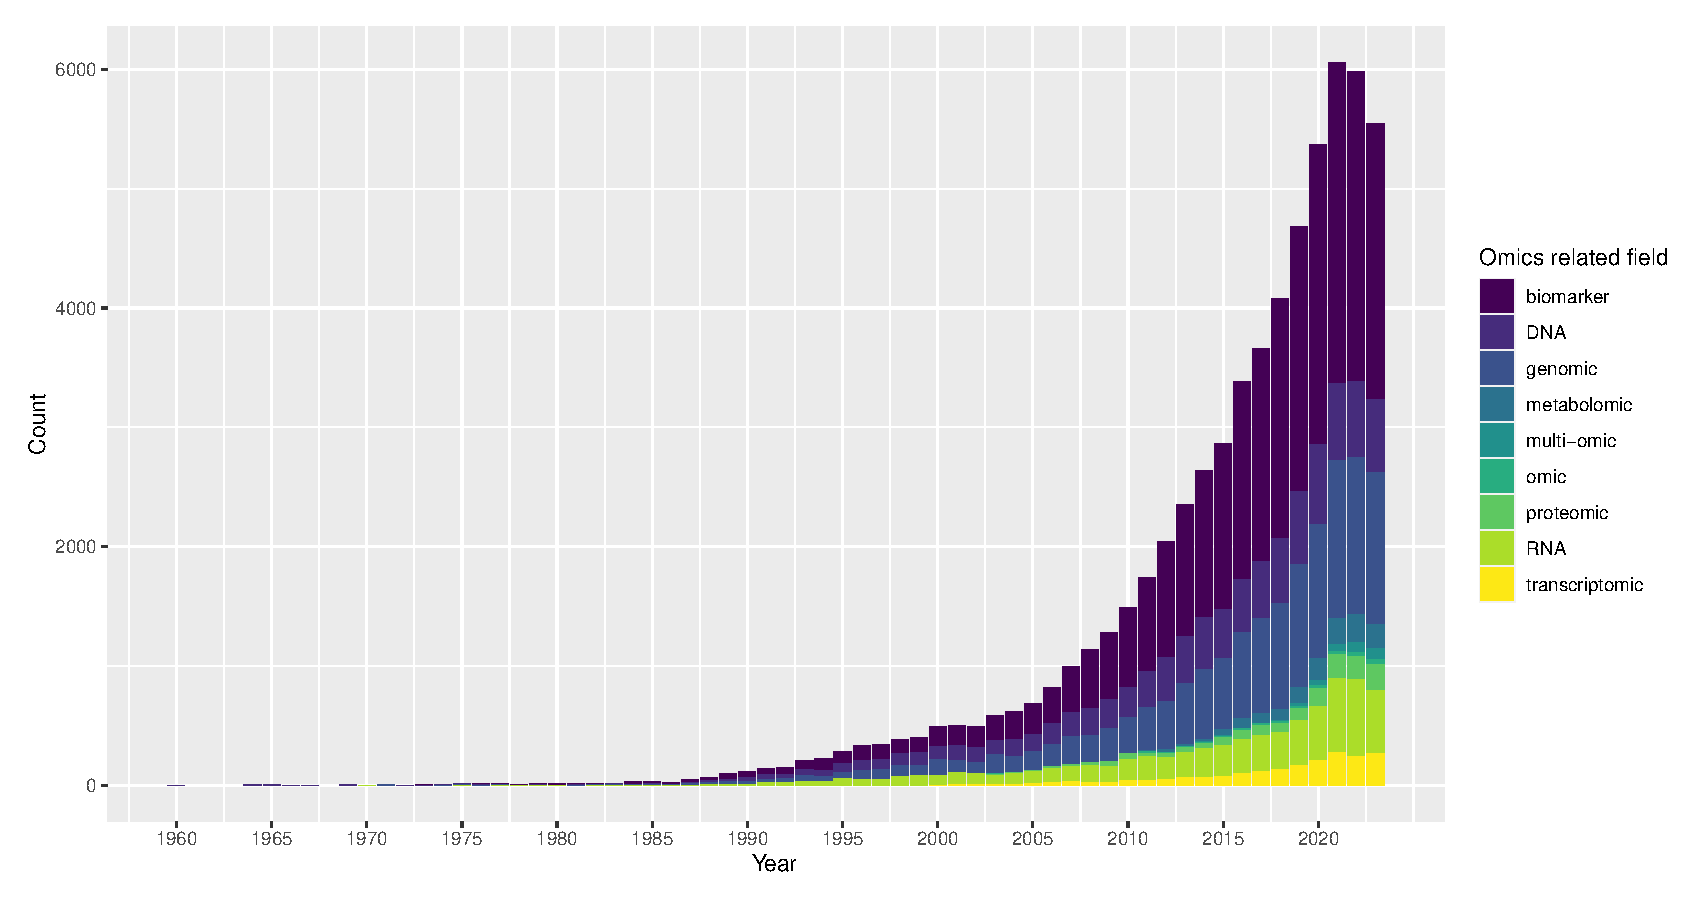
\includegraphics[scale=.4]{pubmed_ggplot.eps}
		\caption{The trend of publications based on longitudinal omics studies within the last 8 decades.}\label{Pubsight1}
	\end{figure}
	
	%\begin{landscape}
	%	\begin{table}
		%		\caption{The summarized introduced  methodologies and applications of longitudinal data in omic studies.}
		%		\begin{tabular}{ccccccccccc}
			%			\hline
			%			entry	&	multivariate	&	response scale	&	application	&	balance	&	time-varying covariate	&	linearity	&	missing	&	high-dimensional	&	software	&	available data\\
			%			\hline
			%			
			%		\end{tabular}
		%		
		%	\end{table}
	%\end{landscape}
	
	
	\begin{sidewaystable}
		\begin{center}
			\begin{minipage}{.7\textheight}
				\caption{The summarized introduced  methodologies and applications of longitudinal data in omic studies.}\label{summary}
				%	\begin{tabular}{\textwidth}{*{11}{>{\RaggedRight\arraybackslash}X}}
					\begin{scriptsize}
						\begin{tabular}{lcllcclcclc}
							\hline
							\rotatebox[origin=l]{-90}{entry}	&	\rotatebox[origin=l]{-90}{multivariate}	&	\rotatebox[origin=l]{-90}{response scale}	&	\rotatebox[origin=l]{-90}{application}	&	\rotatebox[origin=l]{-90}{unbalance}	&	\rotatebox[origin=l]{-90}{time-varying covariate}	&	\rotatebox[origin=l]{-90}{linearity/nonlinear}	&	\rotatebox[origin=l]{-90}{missing}	&	\rotatebox[origin=l]{-90}{high-dimensional}	&	\rotatebox[origin=l]{-90}{presented/used software or code}	&	\rotatebox[origin=l]{-90}{available omic data}\\
							\hline
							\cite{WangMtLMM2013}				&	\cmark	&	continuous		&	pregnancy and HIV-RNA biomarkers										&	\cmark	&	\xmark	&	linear	&	\cmark	&	\xmark	&	
							\cmark																					&	\cmark\\
							\cite{TaavoniArashi2022}			&	\cmark	&	continuous		&	PBCseq biomarkers
							&	\cmark	&	\xmark	&	linear	&	\xmark	&	\cmark	&	
							\cmark																						&		\cmark\\
							\cite{Chengetal2019}					&	\xmark	&	continuous		&	gut microbiome and T1D proteomic
							&	\cmark	&	\xmark	&	nonlinear&\xmark	&	\xmark	&	\href{https://github.com/chengl7/LonGP}{LonGP}				&	\cmark\\
							\cite{waveome}								&	\xmark	&	continuous/count&	CD4, gut microbiome, 
							&	\cmark	&	\xmark	&	nonlinear&\xmark	&	\xmark	&	\href{https://github.com/omicsEye/waveome}{waveome}				&	\cmark\\
							\cite{Liu2018}								&	\xmark	&	continuous&				T1D proteomic
							&	\xmark	&	\xmark	&	linear&\xmark	&	\xmark	& 
							\texttt{R} package \texttt{lme4}				&	\cmark\\
							\cite{HuangFitzmaurice2005}	&	\xmark	&	continuous&				----
							&	\cmark	&	\xmark	&	linear&\xmark	&	\xmark	
							&	\xmark				&	\xmark\\
							\cite{Knudson2021}					&	\xmark	&	continuous/count&				----
							&	\xmark	&	\cmark	&	linear&\xmark	&	\xmark	
							&	\texttt{R} package \texttt{glmm}				&	\xmark\\
							\cite{Ring2022}							&	\xmark	&	discrete					&qPCR result of Ixodes pacificus \textit{Bb} 
							acquisition	&	\cmark	&	\xmark	&	linear&\xmark	&	\xmark	
							&	\texttt{R} package \texttt{glmm}				&	\cmark\\
							\cite{Marshall2000}					&	\cmark	&	continuous/count	&	subunit beta protein 
							&	\cmark	&	\cmark	&	linear/nonlinear&\xmark	&	\xmark	
							&	\xmark	&	\xmark\\
							\cite{Tsiatis1995}					&	\xmark	&	continuous	&	CD4 count and survival 
							&	\cmark	&	\cmark	&	nonlinear&\cmark	&	\xmark	
							&	\xmark	&	\xmark\\
							\cite{WulfsohnTsiatis1997}					&	\xmark	&	continuous	&	CD4 count and survival 
							&	\cmark	&	\cmark	&	nonlinear&\cmark	&	\xmark	
							&	\xmark	&	\xmark\\
							\cite{WangTaylor2001}&	\xmark	&	continuous	&	CD4 count and survival
							&	\cmark	&	\cmark	&	nonlinear&\xmark	&	\xmark	
							&	\xmark	&	\xmark\\
							\cite{Ghosh2011}					&	\xmark	&	continuous	&	HIV viral load with change-point and survival		&	\cmark	&	\cmark	&	nonlinear&\cmark	&	\xmark	
							&	\xmark	&	\xmark\\
							\cite{Vasaikaretal2023}		&	\xmark	&	continuous	&	single-cell and bulk multi-omics		&	\cmark	&	\cmark	&	
							linear&\cmark	&	\xmark	
							&	\href{https://github.com/aifimmunology/PALMO}{\texttt{R} package \texttt{PALMO}}	&	\cmark\\
						\end{tabular}
					\end{scriptsize}
				\end{minipage}
			\end{center}
		\end{sidewaystable}
		
		In  the sequel, we are reviewing the studies their approaches challenged at least one these obstacles. The ideas, techniques,  the scientific question of interest, underlying experimental data and possibly developed computational tools are sketched. In the case of a study targeted more than one of the issues, it is discussed under one the following sections but is also mentioned in the other corresponding sections. Although the statistical approaches are going to be reviewed here, we underscore the studies using omic data. \autoref{summary} summarize the reviewed studies and can be used as a toolbox for underlying experiments or for developing the current methods to cover also a new issue in dealing with longitudinal data. 
		
		\section{Pipelines and platforms}
		Although the work frame of longitudinal studies highly depends on the scientific questions, \autoref{Pipeline1} gives an sketch of it. However, some omics longitudinal studies tried to give a platform from data gathering to the downstream analyses. These platforms may or may not introduce a novel statistical model to deal with the resulting data, but they provide an analysis streamline from data quality control towards the downstream analysis and show the achievements of each steps by answering a scientific question such as ??????. In a zoom-out viewpoint the platforms studies get replaced by suggested pipelines where they less involved with the downstream analysis instead with the structure of the resulting dataset. We take a brief look at some of these platforms and pipelines here. 
		\subsection{Platforms}
		\subsubsection{PALMO}
		A comprehensive platform for longitudinal multi-omics data (\texttt{PALMO}) has been presented by \cite{Vasaikaretal2023} which provides multiple analysis in longitudinal and marginal viewpoints for both the single-cell and bulk multi-omics data. Five analyses were given in PALMO: (1) Variance decomposition analysis (VDA): In longitudinal data analysis it uses a random effect model to decompose the variation of the response variable and employs \texttt{lme4} package in \texttt{R}, (2) Coefficient of variation (CV) profiling (CVP): For bulk longitudinal data it computes the CV of features across the time to distinguish the stable and oscillating features simply by a predefined threshold, (3) Stability pattern evaluation across cell types (SPECT): As a counterpart of CVP for single-cell this analysis computes the CV of individual cell types features and of individual donors. The CV of individual donors are also computed regardless the cell type to create the CV profile. In the same way, the CVs partitioned using a threshold to determine the stable and oscillating features. Using the number of crossing of individual features in cell type-donor combination, the super variables are recognized. Those are not super variable but still variable across all donors are labeled variable across time in cell-types, (4) Outlier detection analysis (ODA): Using the inter and intra-donor correlations the time-points with weaker correlations are labeled as potential outliers. (5) Time course analysis (TCA): Partitioning the the data into individual cell types and individual participants, they employ the \texttt{MAST} package to linearly model the gene expression onto the time. The differential expression gene analysis is derived for the gene expressions with only two time-points. The \texttt{PALMO} package also provides a some visualizations such as circos plot for stability patterns, heatmap of CVs across the time in cell-types, uniform manifold approximation for stable cell-types and many more. 
		
		60 plasma and peripheral blood mononuclear cells (PBMC) blood samples out of 6 healthy donors across 10 weeks were collected to measure the plasma proteins abundances for all, flow cytometry and droplet-based scRNA-seq assays for 24 of the sample of four of the individuals and droplet-based scATAC-seq assays for 18 of these 24 samples which concluded to 27 cell types which those 19 types which have overlap with the 31 cell types reported from the output of \texttt{Seurat} using 472,464 cells were considered. Moreover, 11,191 genes with higher expressions were considered. Considering donors and time-points as random effects, VDA discovered strong inter-donor variations for CBC, PBMC and plasma proteins measurements. It also reported 75 proteins with more intra-donor variation than inter-donor. In both the single-cell data, cell type was added as the random factor which discovered stronger inter-cell type variation than inter and intra-donors variations. In the proteomics data the CVP identified 413 longitudinal variable and 629 stable proteins where the stable proteins are good candidates to be considered as biomarkers. Based on the CVs, the ODA also found weaker intra-donor correlations at week 6 of one of the subjects. For SPECT analysis \cite{Vasaikaretal2023} predefined a threshold and then counted how many times the CV of a gene across time-points is greater than this threshold in the 76 combinations of 4 donors and 19 cell-types. 700 super variable, 2129 super stable, 5750 variable across time in cell-types and 4004 stable across time in cell-types (STATIC) genes where detected. STATIC genes again are potential biomarkers. 
		
		
		
		Inter-donor, intra-donor and inter-cell-types variation.
		
		\subsection{Pipelines}
		
		\section{Unbalanced or missing}
		Although the term `balanced' usually refers to the equal number of observations in each level of factors in simple linear models, a balanced longitudinal study mostly refers to a designed study with common time-points for all the subjects. The source of lack of balance in the sampling design can be the cost of study in some level of particular factors or it could be the rarity of having sample from some individuals which is very common in rare diseases studies. Missing data are also a common reason in achieving unbalanced designs. The usual packages like \texttt{lme}, \texttt{lme4}, \texttt{nlme} in \texttt{R} or procedures like \texttt{MIXED}, \texttt{GLIMIXED}, and \texttt{NLMIXED} in \texttt{SAS} simply omit the rows contain missing values because the structure of missing \citep[see][Sec. 1.3 for completely at random, at random and not at random missing structures]{LittleRubin2002} completely changes the likelihood function. However, the \texttt{Missing Data} task view \citep{Josse2023} provided the list of functions of different packages to deal with missing values without puuting them out. For instance, the \texttt{JointAI} package for Bayesian approach in mixed effect GLM, and more specifically, \texttt{bild} for logistic regression with mixed effects. \texttt{qgtools} also considers the missing structure in LMM specifically for quantitative genetics analyses. 
		\cite{Laird1988} showed how in presence of missing at random (and not completely at random) a bias is imposed into the estimates by misspecification of the dependence structure. Although it seems that in missing completely at random elimination of the missing data row does not impose bias in the decision, this strategy will definitely affect the power or true discovery rate (TDR) of the method. There is a list of imputation methods for missing under different scenarios in \cite{Huque2018}. Overall, \cite{HuangFitzmaurice2005} introduced a model which deals with the unbalanced samples by flexibility in  the model of dependence structure. They decomposed the error of LMM into a weighted combination of a time-dependent error to reflect the dependence across subjects, a serially correlated error and a simple white noise error. Using the iterative likelihood function, the parameters of the model estimated numerically. 
		
		Although most of the methods reviewed here are applicable on unbalanced samples, some of them particularly targeted this issue in the sampling. Most of the methods scrutinized here are are working (admissibly or not) under the unbalanced situation, those studied in this section, deal with this lack, particularly. 
		
		\subsection{LonDA} 
		Returning to the unbalanced structure of longitudinal omic studies, \cite{Marshall2000} introduced longitudinal discriminant analysis (LonDA) of an unbalanced study. LonDA is a classification model which considers the change in the parameter set of distribution of each group across the time. Let $G_j$, $j=1,\ldots,g$ denotes $g$ populations and if the response vector $\mathbf{y}_i$ observed for the subject $i$ on arbitrary times $\mathbf{t}=(t_1,\ldots,t_{n_i})^T$ then the corresponding distribution of $\mathbf{y}_i$ would be $f_j(\mathbf{y}_i;\phi_j(\mathbf{t}))$ where the dimension of density parameters, $\phi_j(\mathbf{t})$, depends on the number of replicates (or dimension of $\mathbf{t}$) per each subject. For prior probabilities $\pi_1,\ldots,\pi_g$, the decision boundary \citep[][P. 102]{ELSII} is 
		\begin{eqnarray*}
			\log \pi_k +\log f_k(\mathbf{y}_i;\phi_k(\mathbf{t})) =\max_j\{	\log \pi_j +\log f_j(\mathbf{y}_i;\phi_j(\mathbf{t}))\}, ~~~~~~~j=1,\ldots,g. 
		\end{eqnarray*}
		If the densities are Gaussian with the same covariance matrices, the decision boundaries are linear. Even in this case, the mean value of the $j$th population, $\boldsymbol{\mu}_j(\mathbf{t};\boldsymbol{\alpha}_j)$ say, can make a nonlinear relationship with the covariates where $\boldsymbol{\alpha}$ is the mean population specific parameter. The rest of modeling procedure returns to the estimation of the parameters. For instance, if $\mathbf{V}_j(\mathbf{t},\boldsymbol{\alpha}_j;\boldsymbol{\theta}_j)$ be the variance matrix of vector $\mathbf{y}$ in the population $j$, where $\boldsymbol{\theta}_j$ is the variance specific parameter of the variance of the population $j$, then regarding \eqref{LMMVar} one can write
		\begin{eqnarray*}
			\mathbf{V}_j(\mathbf{t},\boldsymbol{\alpha}_j;\boldsymbol{\theta}_j)=\mathbf{Z}(\textbf{t};\boldsymbol{\alpha}_j)\boldsymbol{\Sigma}_{\mathrm{rndErr}}(\boldsymbol{\theta}_j)\mathbf{Z}^T(\textbf{t};\boldsymbol{\alpha}_j)+\boldsymbol{\Sigma}_{\mathrm{Err}}(\boldsymbol{\theta}_j),
		\end{eqnarray*}
		where $\mathbf{Z}(\textbf{t};\boldsymbol{\alpha}_j)$ is the design matrix corresponding to the random effect in population $j$. Parameter vectors $\boldsymbol{\alpha}_j$ and $\boldsymbol{\theta}_j$ can be either identical with the mean and variance elements or link them to the covariates. Depends on the homogeneity of $\mathbf{Z}(\textbf{t};\boldsymbol{\alpha}_j)$ and the variance related parameters, $\boldsymbol{\theta}_j$, four estimation situations were expected in \cite{Marshall2000}: 
		\begin{enumerate}
			\item Homoscedastic Model: $\mathbf{Z}(\textbf{t};\boldsymbol{\alpha}_j)=\mathbf{Z}(\textbf{t})$ and $\boldsymbol{\theta}_j=\boldsymbol{\theta}$,
			\item Mean-heteroscedastic model: $\mathbf{Z}(\textbf{t};\boldsymbol{\alpha}_j)$ varies in $j$ but  $\boldsymbol{\theta}_j=\boldsymbol{\theta}$,
			\item Variance-heteroscedastic model: $\mathbf{Z}(\textbf{t};\boldsymbol{\alpha}_j)=\mathbf{Z}(\textbf{t})$ but $\boldsymbol{\theta}_j$ varies in $j$, and
			\item Fully-heteroscedastic model: Both the $\mathbf{Z}(\textbf{t};\boldsymbol{\alpha}_j)$ and $\boldsymbol{\theta}_j$ vary in $j$. 
		\end{enumerate}
		\cite{Marshall2000} studied the subunit beta measurements of 174 pregnant women over 2 years in a private obstetrics clinic in Santiago, Chile. The data were unbalanced since there were only one measurement for 30\% of subjects, two for 31\%, three for 33\%, and 6\%  with more than three measurements. The subunit beta is used as a biomarker in this study to discriminant the samples with normal/abnormal delivery. Prior probabilities were the proportion of each group in the sample. The response variable was $\log$ subunit beta measurements and the response of the $i$th subject at time $t_{ik}$ when it belongs to $j$th group in the sample, $y_{i,t_k}^{(j)}$ for instance under the Mean-heteroscedastic model follows
		\begin{eqnarray*}
			y_{i,t_k}^{(j)}=\frac{\alpha_{j1}+b_{ij}}{1+\alpha_{j2}e^{-\alpha_{j3}t_{ik}}}=\varepsilon_{it_{ik}j}, 
		\end{eqnarray*}
		where here, $i=1,\ldots,174$, $j=1,2$ and $t_ik$ is the $k$th time of measurement for subject $i$ where $k=1,\ldots,n_i$. In this study, $n_i=1,2,3,>3$ and suggests the notation $\boldsymbol{\alpha}_j=(\alpha_{1j},\alpha_{2j},\alpha_{3j})$. The remaining three models can be written in the same way and the fitted models chose the fully-heteroscedastic model based on the deviance test which confirms the longitudinal effects in both the mean and variance of the $\log$ subunit beta measurements in two groups. Although there is no restriction of using the same method on the multivariate case, \cite{Marshall2009} specifically discussed the bivariate case of this model with considering the missing completely at random structure applied on the  Estradiol and $\beta$-HCG concentrations but using the 161 subjects and it is mentioned that they employed \texttt{NLMIXED} procedure from \texttt{SAS} to estimate the parameters. The same data under fully-heteroscedasticity assumption using the nonlinear hierarchical classification were studied by \cite{delaCruzMesia2007}. 
		
		
		
		
		
		\cite{Colosimo2012} 
		
		
		
		
		
		
		\section{LMM based approaches}
		In previous sections we see the impact of the essential model \eqref{LMM} in the analysis of longitudinal data. Most (??????Check most of them or all of them before this sentence) of the analysis used the derivatives of this model in confronting the longitudinal measurements. However, the direct use of LMM still answers important scientific question in the field of longitudinal omics data. After a brief review of this studies we take a look at a family of extensions to LMM called GLMM and its usage in omics data.
		\subsection{Continuous value LMM}
		\subsection{Discrete value response}
  The longitudinal omics studies are mostly based on the abundances of omics features where in many studies these counts are transformed into relative abundances. Even in the count cases, the normal approximation to the response Poisson or negative binomial distributions is a common approach. However, this is not the case in the derivatives of omics studies such as CD4 or T-cell counts. Moreover, the over-dispersion and the zero-inflation of the response variable makes the normal assumption far from the model. These cases specifically are analyzed based on discrete distribution and inevitably the simple linear models are not helpful anymore.
		\subsubsection{GLMM}
		The only GLMM used study based on omic data that we are going to review is \cite{Ring2022} where it is a repeated measurement study which is a particular case of longitudinal sample with eliminating the lag effect. On the other hand, repeated measure models consider the same mutual correlation between the measurements collected from the subject. \cite{Ring2022} studied the influence of larval host bloodmean on \textit{Borrelia burgdorferi} (\textit{Bb}) infection of Ixodes pacificus ticks. To this end, the raised larvae on western fence lizards (\textit{S. occidentails}) from China camp State Park in Marine, CA and laboratory deer mice (\textit{P. maniculatus}) were collected and sent to a laboratory at San Fransisco State University. The molted nymphs partitioned into three groups and one part was sent to Indiana University while the remaining two sets stayed in the lab. The resulting ticks are sent to get fed from three groups of 17, 3 and mice in three partitions, respectively, where mice were inoculated intradermally withh $100\mu l$ of \textit{Bb} culture, $10^3$ total spirochetes for partition one, $10^5$ spirochetes for partition two and $10^4$ for partition three and tested positive for \textit{Bb} acquisition. A total of 36 and 46 \textit{Ixodes pacificus} nymphs collected from lizard and mice-fed in the three partitions and planted on \textit{Bb} acquired mice. Simultaneously, a total of 12 nymphs got fed on non \textit{Bb} acquired mice as control. DNAs from $Bb$-fed nymphs were examined by qPCR for \textit{Bb} acquisition where \textit{Bb} CA4 cultures were supposed t ocreate silution sereis of \textit{Bb} DNA standards for qPCR. The responce variable is the binary variable of testing positive/negative for the qPCR test. They used the model \eqref{GLMM} with Bernoulli distribution and used the \textit{Bb} infection of the host, the larval hosted animal (lizard/mice) and acquisition doses as the fixed factors and the index of host mice and the partition number as the random effects. The results emphasized the significant positive effect of lizard larval on the odd of positively \textit{Bb} testing. The model also stated that the host bloodmeal may shape vector competency of ticks across at least one life stage transition. However, the results have not been followed by a post-hoc testing to determine which life stage transition caused this significance in the model. 
		
		\subsubsection{Differential expression analysis}
		The most part of the attention in Differential expression analysis (DEA) is to study the change of the mean function as a function of time. A very primary approach in this viewpoint is simple generalized linear models where the time index is considered in the model as class variable. Therefore, one of their main assumptions is the independence of the observations in different time-points. However, some of DEA models simultaneously deal with the dependence structure of collected sample out of the same subject along the time. Among them, some investigate the change in the variation of the data alongside the time change by the effect of the mean function on the variance. For instance in the exponential dispersion family this can be done by looking to the dispersion parameter as a hyper-parameter which links the variance of the response variable to its mean. 
		
		\cite{Anders2010} developed \texttt{DESq1} package in \texttt{R} which has been particularly designed for the longitudinal negative binomial responses. Let $K_{ij}$ be the the number of genes of type $i$ in sample $j$. The package assumes that $K_{ij}\sim NB(\mu_{ij},\sigma^2_{ij})$ where the mean $\mu_{ij}$ is the product of size factor of $j$th sample, $s_j$, and a quantity related to the condition of the sample,$q_{i,\rho(j)}$ where $\rho(j)$ indicates the sample condition. Te time effect enters into the account from here. The variance $\sigma_{ij}^2=\mu_{ij}+s_j^2\nu_{i,\rho(j)}$ is also determined by the smooth function $\nu_{i,\rho(j)}=\nu_{\rho}(q_{i,\rho(j)})$. The provided package uses the intrinsic estimation of the size factor and the condition-dependent quantity, $q_{i,\rho(j)}$. Estimation of $\nu_{\rho}(q_{i,\rho(j)})$ requires a considerable time of replications which usually does not happen in the longitudinal studies. Therefore, the package uses local regression method to fit this function and hence estimate the variance term. \texttt{DESq1} package also provides testing for $H_0:q_{iA}=q_{iB}$ where $A$ and $B$ are two different conditions. If the observed counts under these two conditions are $K_{iA}=k_{iA}$ and $K_{iB}=k_{iB}$, then using the negative binomial distribution under the null hypothesis, the $p$-value of the test is reported mutually on conditions and separately for each gene. This method applied on (1) the paired-sample of RNA sequence of fly embryos data, (2) RNA sequence on replicates of \textit{Saccharomyces cerevisiae} cultures for two library preparing protocols, \textit{dT} and \textit{RH}, where three sequences were extracted under each protocol \citep{Nagalakshmi2008}, (3) ChIP-Seq of mapping NF$\kappa$B and PoIII binding sites in ten human, replicated twice on each individual \citep{Kasowski2010}, and (4) four Tag-seq out of \textit{glioblastoma}-derived neural stem (GNS) cell lines and two sequences out of neural stem (NS) cell lines \citep{Engstrm2012}. The first and the latest studies were used also for no replication case by restricting the data to only to one sample from each condition. The low sample size will be reflected in the overestimation of the variance function. 
		
		
		
		\begin{enumerate}
			\item \cite{Bach2021} used LMM to investigate the circadian variation of urinary cell-free DNA and methylation levels of cancer-related genes for non-small cell lung cancer patients. 
			\item \cite{ChenLi2016}
			\item \cite{Vasaikaretal2023}
			\item \cite{Bernardesetal2020}
			\item \cite{Marsetal2020}
			\item \cite{SchsslerFiorenzaRoseetal2019}
		\end{enumerate}
		
		
		
		\subsection{Bayesian approach on LMM and GLMM}
		
		
		Employing the Bayesian approach in longitudinal data analysis is mostly happen through two main ideas: (1) A Bayesian statistical model \citep[see][Page 9 for the definition of the parametric version]{Robert2007} which considers a prior distribution on the parameters of a parametric statistical model and (2) a machine learning approach in considering parameters as a latent variable \citep{Blei2017}. Using either approach tends to the computational problem of posterior computation. 
		
		The problem of estimating the parameters of LMM in Bayesian approach has been widely studied and performed in different softwares such as \texttt{brms} \citep{brms2021},  \texttt{blme}, \texttt{DESeq2} \citep{Love2014}, \texttt{JM} \citep{Rizopoulos2010}, \texttt{JMbayes} \citep{Rizopoulos2016}, \texttt{bmrarm} \citep{Seedorff2022}, \texttt{APML0} \citep[see the implementation for longitudinal data in][]{Xu2020}, and \texttt{JSM} \citep{Xu2020JSM} packages and, \texttt{BayesselectGLMM} function in \texttt{R} \citep{Ariyo2021}, \texttt{Time-Varying Group SpAM} code in \texttt{Matlab}\citep{MarchettiBowick2016}, and \texttt{PairedFB} \citep{Bian2018}, and \texttt{Stan} \citep{Sorensen2016} stand alone softwares. There is also a guideline to use \texttt{winBUGS} package in \texttt{R} for general framework of Bayesian GLMM which can be used for longitudinal data. 
		CD4 have been widely used as a biomarker indicator of HIV infection which usually is considered as a time-varying index \citep{Tsiatis1995}. The clinical data of studying the efficiency of \textit{ddl} drug is three different doses were used by \cite{LAVALLEY1996} where 650 subjects randomly attributed to one of the three doses and the baseline measures of CD4 at the start of the study 
		
		
		\subsection{Bayesian approach on trajectories}
		%GP approach in facing the longitudinal data instead of the classic general linear mixed effect models, was introduced by \cite{Quintana2016}. The idea is replacing the simple white noise error in model \eqref{LMM} by an autoregressive noise and more generally with any GP with known structure of covariance function but unknown parameters. Usually, this known covariance structure is induced in the model by a kernel function or a combination or multiplication of kernel functions. 
		Interdomain GPs is based on considering the time-dependent responses of each subject as a path of a continuously indexed Gaussian process realized at a countable (and sparse in most of the cases) point. The decision making is to find the posterior distribution of the function in all the domain given the observed points. Precisely speaking, the observed values $\mathbf{y}_i=(y_{i1},\ldots,y_{in_i})^T$ at time-points $\mathbf{t}_i=(t_{i1},\ldots,t_{in_i})^T$ for given covariate values $X_i=(\mathbf{X}_{it_1},\ldots,\mathbf{X}_{it_{n_i}})\in\mathcal{X}$ 
		are considered as realized values of the model $\mathbf{y}_i|X_i,\mathbf{t}_i\overset{ind}{\sim}N(f(X_i),\sigma^2)$ for $i=1,\ldots,N$ where $f$ is a zero mean Gaussian process with unknown covariance (kernel) function. This assumption provides us the likelihood function. Therefore, the structure of dependence in the repeated measurements of a subject is modeled via the kernel function. The problem in this state is a nonparametic problem of estimation of the kernel function but in practice, it is usual to solve the parameters of the given kernel function and then, choose the family of kernel using information criterion like AIC or BIC. 
		By considering Gaussian process prior for $f:\mathcal{X}\rightarrow\mathbb{R}\sim \mathcal{GP}(0,k(\cdot,\cdot))$ where $k:\mathcal{X}\times\mathcal{X}\rightarrow\mathbb{R}$ is a positive definite kernel function, the posterior distribution of $f|\mathbf{y},X$ as a posterior for the functional parameter $f$ is computed \citep{vanderWilketal2020}. Let $X\subset \mathcal{X}$ be a finite countable set made out of the disjoint values of the covariates at different time-points. Therefore, the problem is computation of the posterior $p(f(\cdot)|Y,X)$ for whole the domain of the function $f$. One can categorize this approach based on the last statement into a nonparametric problem. \cite{Chengetal2019} introduced the additive model of GPs approach called LonGP, by considering $f=f^{(1)}+\ldots+f^{(D)}$ which is simply distributed as $\mathcal{GP}(0,k^{(1)}+\ldots,k^{(D)})$ where $k^{(\delta)}$, for $\delta=1,\ldots,D$ are different kernel functions with known structures but unknown parameters. The provided Matlab based code considers squared exponential and periodic kernels for continuous covariates and constant, binary and categorical kernels for categorical covariates (factors) and also any valid bi-product of these stationary kernels. They also considered a non-stationary kernel for better covering the real life data. See \cite{Plate1999} for sum of univariate and multivariate kernels and \cite{Duvenaudetal2011} for more complicating kernels. However, the model may conclude to multiple use of the same kernel but with different parameter estimates. A general form of the additive model is the one presented by \cite{waveome} where both the sums and multiplications of different kernel functions are considered in the model selection. Although \cite{waveome} uses BIC for model selection, \cite{Chengetal2019} use one-leave-out and stratified cross-validations and Bayesian bootstrap. 
		
		\cite{Chengetal2019} employed LonGP for the metagenomic data set from 758 stool samples out of 222 children in Estonia, Finland and Russia collected from born to age three of the subjects. They aimed to answer the question of the effect of socio-economic status on the gut microbiome. Breast feed status (yes/no), type of born(Caesarean/vaginal), and country were three factors and age was the only continuous covariate of the study. Considering 394 pathways in the stool samples, define $c_{ij}$ as the number of reads mapping to genes in the $j$th pathway and $i$th sample where $j=1,\ldots,394$ and $i=1,\ldots,785$. If $C_i$ is the total number of reads in the $i$th sample, they considered $\log_2\left(c_{ij}/C_i \mathrm{median}(C_1,\ldots,C_{785})+1\right)$  as the response variable. The model concluded the results of \cite{Vatanen2016} which had stated that the gut microbiome of Russian children were significantly less enriched compare to two other countries. 
		
		LonGP was also applied on the proteomics data set of 11 children who developed type 1 diabetes (T1D) and 10 control children. The data contain the nine times measurement of the  intensity of more than 2000 proteins in plasma samples where the last measurement for case samples collected at the time of T1D diagnosis. Since the sample is balanced in replication, \cite{Liu2018} used the LMM by considering the age of the subjects as the only fixed effect and the normalized log abundance of the proteins as the responses to find the significantly effective proteins (biomarkers) in development of T1D. In the LonGP analysis of the same data, the sero age of the individuals which is the first age that autoantibodies are detected alongside the gender, group and ID were imported as new covariates into the model. 38 proteins are significantly correlated with the group variable via the model where 18 proteins of this list have not been recognized in the previous study. Moreover, 47 proteins also have correlation with the seoconverssion age. 
		
		
		
		
		\section{Survival, dropout and sparsity}
		In many omic studies particularly for sever diseases cases, not all the subjects remain by the end of panel study. Some of them change the treatment regime by change in their health status at the middle of study, some leave the study because they decide not to corporate or they found themselves completely treated or because of death. Either of cases of leaving provides its specific consideration in the model which usually put forward the time of leaving into account. This time is usually considered as continuous and if the aim of study is focused on this time (for instance in healing time or mortality time) survival models are hired. A wide range of studies in longitudinal models attributed to the joint modeling of the underlying longitudinal model and the time-to-event. 
		\subsection{LMM alongside Cox regression}
		One of the most popular joint models for longitudinal data of treatment efficiency studies is considering the data as a realization of a repeated measure or sparse stochastic process jointly with studying the effect of covariates (usually treatments) on the time of level-crossing of the response variable (usually the biomarker) or dropout. \cite{Tsiatis1995} is one of the first studies in this framework which studied the effect of Zidovudine (ZDV) on the CD4 counts and simultaneously examined whether CD4 counts serves as a surrogate marker for survival of HIV patients or not. The study is based on a double-blind placebo-controlled trial of 281 advanced HIV patients 144 of those randomly received a $250mg$ of ZDV every four hours and the rest of them received placebo and CD4 counts were measured periodically for each subject. The response variable of CD4 count in the previous model is now using as the covariate of the Cox regression which requires a complete history of the time dependent CD4 while we have only access to the values of it on some specific times. Let $y_{ij}$ be the CD4 count of patient $i$ at time $t_{ij}$ were measured and denoted by  for $i=1,\ldots,281$ and $j=1,\ldots,n_i$. \cite{Tsiatis1995} assumed that $y_{ij}$ follows a LMM like \eqref{LMM}. If $T$ denotes the survival time, we hope to model $T^*$ using the CD4 ($y$) and hence the covariates of the LMM which is treatment here. If we denote the left censoring time by $C$ which is the time that individual leaves the study because he/she gets recovered, changes the treatment plan or passes out, we practically observe $T=\min\{T^*,C\}$. The aim of Cox regression is to model $T$ using the hazard rate function $\lambda(t|\mathbf{y})=\lambda_0(t)g(\mathbf{y},\boldsymbol{\gamma})$. The big issue in this way of modeling is the missing stricture which in this particular case the probability of missing is higher for the patients with lower level of CD4 that is a nonrandom missing implying a bias into the estimation. The joint estimation of the random effect (which is the linear effect of time here) derived by the empirical Bayes estimate given by \cite{LairdWare} and adjusted for missing data. The extended version of this model with considering the change-point is given in the next section. \cite{Tsiatis1995} study confirmed that ZDV significantly changed the Kaplan-Meier survival curve between case and control groups and subjects who received ZDV have substantially greater CD4. This joint model, simultaneously confirms that CD4 is an admissible biomarker while the use of ZDV significantly changes its values. The \texttt{brms} package in \texttt{R} can provide the estimation of the parameters from this nonlinear model without considering the missing. This is the  The resulting estimations must adjusted for missing using the method introdiced by \cite{Tsiatis1995}. Compare to the partial likelihood used in this model to estimate the Cox regression parameters, \cite{WulfsohnTsiatis1997} introduced a more computationally efficient EM algorithm to estimate the Cox regression parameters as well as the LMM parameters and applied it on the same data which tended to the similar results. 
		
		\subsection{Integrated Ornestein-Uhlenbeck random effect}
 		The two stage method of \cite{Tsiatis1995} has been extended to include time-varying coefficients for CD4 count studies. The data of 115 men those HIV antibody test changed from negative to positive before June 15, 1996  from seroconverters in the LA center were used where the median of the last negative time and the first positive time was considered as the infection time. The CD4 measurements 6 months following the infection date were excluded because it imposed a sudden change in the slope of the CD4 counts. The time to event (disease or last visit) starts 6 months after the infection time and $y_{ij}$ is $\sqrt[4]{\mathrm{CD4}}$ of the $i$th subject at time $t_{ij}$. \cite{WangTaylor2001} introduced the model 
 		\begin{eqnarray*}
 			\left\{
 			\begin{array}{lcl}
 				y_{ij}&=&\psi_i(t_{ij})+\varepsilon_{ij},\\
 				\psi_i(t)&=&a_i+bt+\mathbf{X}_i\boldsymbol{\beta}+W_i(t),
 			\end{array}\right.
 		\end{eqnarray*}
 		where $a_i$ is the random intercept, and $W_i$s are independent Ornestein-Uhlenbeck processes. The proportional hazard model is $\lambda(t|\phi_i(t),\mathbf{X}^*)=\lambda_0\exp(\gamma\psi_i(t)+\mathbf{X}^*\boldsymbol{\beta}^*)$ where $\mathbf{X}^*$ is the possible extra covariate for the Cox regression and $\boldsymbol{\beta}^*$ is the corresponding coefficient. The full Bayesian estimate and an efficient MCMC algorithm to estimate the corresponding parameters were also given. In the clinical data there is range from 1 to 32 times of visits for the subjects therefore the sample is highly unbalanced. The average $\sqrt[4]{\mathrm{CD4}}$ before infection time and the age at the time of infection are considered as the fixed effect for the LMM part and the covariates of the Cox regression where in presence of $\psi_i$ we can expect the insignificant effects of these covariates in the Cox regression. Based on the results the decrease in the CD4 and its effect on the survival odd justified by the negative estimated $b$ and $\gamma$, respectively. This method 
 		highly decreased the MSE compare to the simple use of the random effect model. 
 		
 		\cite{WangTaylor2001}
		\subsection{Change-point detection model}
		Plasma HIV RNA data from AIDS Clinical Trials Group (ACTG) 398 study \citep{Hammer2002} were generated in a double-blinded case-control study to compare a single protease inhinitor (PI) and double-PI regimens as two well-known treatments for HIV. The viral load of 481 patients were followed at at 0, 2, 4, 8, 16, 24, 32,
		40, 48, 56, 64 and 72 weeks to discover the effect of regimes in virologic failure after 24 weeks. The sample design is unbalanced due to missing and dropout of subjects. The viral load, of patient $i$ at time $t_{ij}$ were measured and denoted by $y_{ij}$ for $i=1,\ldots,491$ and $j=1,\ldots,n_i$. The results of each patient were mapped in a trajectory map as a function of time. The results showed that the resulting function, behaves differently in different time intervals. Therefore, \cite{Ghosh2011} in one hand considered the model 
		\begin{eqnarray*}
			y_{ij}=\mathbf{X}_i\boldsymbol{\beta}+b_{i0}+b_{i1}t_{ij}+\sum_{l=1}^{L}\alpha_{il}(t_{ij}-\tau_l)_++\varepsilon_{ij}\coloneqq \psi_{i}(t_{ij})+\varepsilon_{ij},
		\end{eqnarray*}
		where the random effect part is linear in time but the last term lets a piecewise linear behavior on $L$ knots where considered here as the change-points. The random error here is not white noise here instead $\varepsilon_{ij}\stackrel{iid}{\sim}N(0,\sigma^2/\eta_i)$ which gives the researchers more flexibility to conclude the results subject-related. The hazard of dropout of the $i$th subject at time $t$ is modeled through the Cox proportional model, i.e., $\lambda(t|\psi_i)=\lambda_0(t)\exp(\gamma\psi(t))$ where $\lambda_0(t)$ is a predefined step function and bigger $\gamma$ implies higher dropout rate. The estimation of the parameters obtained by a full Bayesian model using MCMC. They also considered the missing data in the model on missing at random structure. Treatment factor in four levels (three dual-PI arms and the placebo-PI arm) and NNRTI are fixed effects covariates. The results concluded to significant effect of NNRTI and the positive dropout rate on the RNA viral load. 
		
		
		
		
		
		
		\begin{enumerate}
			\item \cite{Ghosh2010} employed a multiple change-point model to cluster the RNA data. 
			\item \cite{Wu2012}
		\end{enumerate}
		
		
		\section{Multivariate outcomes}
		The main feature of omic data is measuring multiple omic features simultaneously which we expect most of them are correlated. Although deriving the study independently for each measured response variable in the most of the times answers the research questions, a considerable information may be ready to get extracted in the correlation between outcome variables. There is a comprehensive review by \cite{VerbekeetalReview2014} on the possible approaches on multivariate longitudinal responses and we review those with direct applications on omic data or biomarkers. For this section, let we have $p$ outcomes measured at $n_i$ time-points or replicates for subject $i=1,\ldots,N$ and denote the collected data for subject $i$ by $Y_i=\left[\mathbf{y}_{i1}|\ldots|\mathbf{y}_{ir}\right]$, an $n_i\times r$ matrix where $j$th column is $\mathbf{y}_{ij}=\left(y_{ij,1},\ldots,y_{ij,n_i}\right)^T$. The whole data is an $i:1\ldots,N\times j:1\ldots r\times t:1\ldots n_i$ array where $n_i$ is the number of time-points subject $i$ is measured. The measurement error is denoted by $\mathcal{E}_i=\left[\boldsymbol{\varepsilon}_{i1}|\ldots|\boldsymbol{\varepsilon}_{ir}\right]$ where 
		$\boldsymbol{\varepsilon}_{ij}^T=\left(\varepsilon_{ij,1},\ldots,\varepsilon_{ij,n_i}\right)$.
		
		\subsection{MtLMM}
		The multivariate $t$ linear mixed model (MtLMM) considers outcomes as a random vector sample of a multivariate $t$ distribution which gives more flexibility on the tail feature of the symmetric responses by considering missing values, whether at random or not at random missing in the model estimation \citep{WangMtLMM2013}. MtLMM models the row-wise vectoriziation of $Y_i$ which is $\mathbf{y}_i\coloneqq vec(Y_i)$. The model is matrix form of \eqref{LMM} in for of 
		\begin{eqnarray*}
			\mathbf{y}_i=X_i\boldsymbol{\beta}+Z_i\mathbf{b}_i+\boldsymbol{\mathcal{E}}_i,
		\end{eqnarray*}
		where $X_i=diag\{X_{i1},\ldots,X_{ir}\}$ is a block-diagonal matrix made out of sub-design $n_i\times p_j$ full-rank matrices $X_{ij}$. Therefore, this model also considers the option of using different number of covariates ($p_j$) for each outcome. In the same way, $Z_i$ is a blocked diagonal matrix of $n_i\times q_j$ random effect matrices. In this model, the measurement error is $\boldsymbol{\mathcal{E}}_i\coloneqq vec(\mathcal{E}_i)$ and the random vector $\left(\mathbf{b}_i^T,\boldsymbol{\mathcal{E}}_i^T\right)^T$ is distributed as a $q_.+n_i$-variate central $t$ distribution with scale matrix $diag\{D,R_i\}$ and $\nu$ degree of freedom where $q_.=\sum_j q_j$. Here, $D=[D_{jj'}]$ is a block matrix made out of $q_j\times q_{j'}$covariance matrix $cov(\mathbf{Z}_{ij},\mathbf{Z}_{ij'})$ where $\mathbf{Z}_{ij}$ is the $i$th row of the design matrix of the random effects corresponding to the $j$th outcome. In the same way, $R_i$ is the $rn_i\times rn_i$ covariance matrix of the random error corresponding to all the measurements collected from subject $i$ and for the sake of parsimonious and model identifiability it is considered in form of $R_i=\Sigma_{Err}\otimes C_i$ and $C_i$ is the induced time-dependence correlation in form of damp exponential correlation (DEC)structure. This structure adds two correlation parameters to the model. The user can also consider different correlation parameters for different outcome which can considerably increase the number of parameters and hence the AIC of the model. We consider the complicating form of the model as its feature since it gives the users a wide range of inter and intera-dependence structure. Writing the likelihood function for full (observed and missing) values, instead of simple EM algorithm, \cite{WangMtLMM2013} introduced an efficient alternating expectation-conditional maximization (AECM) algorithm for estimation of the parameters. They essentially used the AECM algorithm hybridizing with Fisher score method. The random effect is estimated using the the likelihood given the observed values using an empirical Bayes approach. The result is not a Bayes estimate of the random effect and the estimator uses the empirical Bayes method \cite[][Page 78]{VerbekeMolenberghs2009} as shrinkage estimator of the random effects. 
		
		The panel data consist of 161 young women collected from a private fertilization obstetrics clinic in Santiago, Chile. Two biomarkers estradiol and $\beta$-HCG concentrations were measured during the first three month of pregnancy. At the end, the pregnancy happened either normally (124 patients) or abnormally (37 patients). Totally, 348 measurements collected from these 161 patients for each variable and logarithmic transformation applied on the response variables. The covariates are rescaled time and squared value of time alongside the pregnancy group factor. AIC-wise the MtLMM with DEC correlation structure and BIC-wise, MtLMM with AR(1) correlation structure dominated other types of models in describing the variation of the data. 
		
		The other analysis is studying the bivariate responses of HIV-1 RNA (count/ml) in seminal and blood of patients in HIV-RNA AIDS studies from Seattle, Swiss and UNCCH cohorts. The data were collected out of $N=149$ subjects divided into two groups of patients who were receiving a therapy (14=106 patients) and those with no therapy or unknown therapy method (43 patients). The covariate are scaled time, baseline age, baseline CD4 and two factors consists of group and cohort.  MtLMM with DEC correlation structure achieved lower AIC compare to other types of correlation and also compare to simple LMM with normal distribution. The same model was studied by \cite{TaavoniArashi2022} by penalizing the likelihood to cover the high-dimensional problems. However, the model and the provided codes do not support the missing values. 
		
		
		
		
		
		\section{Miscellaneous obstacles}
		
		\subsection{Low replication}
		The high load of replication and regularity in longitudinal studies give the researchers to fit a variety of models by considering the omic features as dependent variable and time as the dependent variable. For instance, \cite{Vaas2012} provided a framework to fit user-definite curves to phenotypic features. A usual method to look at the phenotype of an organism is characterizing its growth behavior under a specific condition over time. In Phenotype MicroArray data, the number of phenotypes is considerably large (not as large as the number of a normal omic data) but the number of measurements replicate is also high in this system which is a good news because not only there is no sparsity problem, the regular observations also guarantee obtaining balanced data. In this type of studies the computational cost could be addressed as a problem because the large number of replication increases the dimension of the covariance function of the random effect for each phenotype if the underlying analysis approach is using simple LMM separately for each phenotype. Instead, curve fitting methods are employed in these kind of studies to map the phenotype onto the time. The motivating dataset in \cite{Vaas2012} is two times measurements of two strains of two bacteria species \textit{Escherichia coli} DSM $30083^T$, \textit{E. coli} DSM $18039 = K12$, \textit{P. aeruginosa} 429SC under LB medium condition and \textit{Pseudomonas aeruginosa} DSM 1707 under agar condition for about 24h where measured on GEN III MicroPlates in the PM modus over 91h and measured in ten technical replicates.  2 datasets$\times$ 4 strains $\times$ two biological replicates $\times$ ten technical replicates $\times$ 96 substrates tend to $7680$ individual time-dependent measurements. \texttt{smooth.spline()} function in \texttt{R} was used to fit the cubic spline to the curves. The reason of fitting the curve instead of analyzing the time-dependent data in a linear-type model is using the estimated area under each curve (AUC) as a description for the cell growth and the reason for comparison of AUCs instead of the parameters of the fitted curves is summarizing whole estimation procedure for each sampling condition and variable into AUC which in this case they also observed that AUC is more correlated with one of the interested parameters, growth rate say. Hence, they concluded that the restricted number of employed data points in curve fitting and symmetry assumption around the inflection point considered by Phenotype MicroArray system native analysis software, \texttt{OmniLog}\textsuperscript{\tiny\textregistered} tend to bias in the estimations and to neglect some part of information stored in the data. 
		
		Although even the paired sample studies as studies with low replications can be also considered as longitudinal models, the number of replication is one the concerns in omic data. It can affect the study by taking it into the high-dimensional literature since for instance in DNA reads there is no guarantee that the structure of the correlations keep same in all the genes. The intrinsic estimators of the hyper-parameters in \cite{Anders2010} requires considerable replication at least in one of the sampling conditions since it essentially uses the mean of reads to estimate the size factors and sample condition  quantity. However, the method still works under the assumption of having no true differential expression for most of the genes when there is no replication at neither of the conditions. But consider in mind that the sample means used in the estimation procedure all will have only one term. \cite{Love2014} and \cite{Wu2012} deal this problem by use of Bayesian estimates of negative binomial and Poisson regression parameters, respectively. 
		
		
				
		\subsection{nonparametric}
		\begin{enumerate}
			\item \cite{Metwallyetal2022}
		\end{enumerate}
		
		\subsection{Integration}
		\begin{enumerate}
			\item \cite{Sperisenetal2015}
			\item \cite{Bodeinetal2021}
			\item \cite{Stanberryetal2013}
		\end{enumerate}
		
		\subsection{Random forest}
		\begin{enumerate}
			\item \cite{HuSzymczak2023}
		\end{enumerate}
		
		\subsection{Clustering, abundance change network modelling}
		\begin{enumerate}
			\item \cite{Kodikaraetal2022}
		\end{enumerate}
		
		\subsection{Dynamic modelling }
		\begin{enumerate}
			\item \cite{Dingetal2019}
		\end{enumerate}
		
		
		
		\subsection{High-dimensional}
		\begin{enumerate}
			\item \cite{Moretal2022}
			\item \cite{McKennanNicolae2022}: CBCV-CorrConf family of algorithms.
		\end{enumerate}
		
		\subsection{SVM}
		\begin{enumerate}
			\item \cite{Zhouetal2019}
		\end{enumerate}
		
		
		
		
		
		\subsection{Used methods}
		\cite{Mishraetal2022} employed a variety of methods to explore the longitudinal cohort study for inflammatory bowel disease (IBD) patients using two independent cohorts under anti tumor necrosis disease (TNF) infliximab or adalimumab and the cohort those received  vedolizumba as a therapy control. The study focusses on the RNA and DNA methylome of the subjects. The subjects were fully observed within the observation time interval and pairwise comparison at each time-point as well as longitudinal approaches were used to discover the differences in the gene expressions. The longitudinal analysis was derived through the ImpulseDE2 model \citep{Fischer2018}
		
		
		
		
		
		
		
		%
		%
		%Linear Models:
		%\begin{enumerate}
		%	\item Linear Model approach:
		%	\begin{itemize}
			%		\item \cite{MolenberghsVerbeke2007}
			%		\item \cite{Pan2001}
			%		\item \cite{LinZhao2009}
			%		\item \cite{Lippertetal2011}
			%		\item \cite{Liangetal1992}
			%		\item 
			%	\end{itemize}
		%	\item Dimensionality Reduction:
		%	\begin{itemize}
			%		\item \cite{Alteretal2000}
			%		\item \cite{QiaoWang2010}
			%		\item \cite{LeeSeung1999}
			%	\end{itemize}
		%	\item Machine Learning:
		%	\begin{itemize}
			%		\item 
			%	\end{itemize}
		%\end{enumerate}
		
		
		
		
		
		
		
		
		
		
		
		
		
		
		
		
		
		
		
		
		
		
		%
		%\section{Mixed model approach}
		%\subsection{Repeated measure case}
		%Let we have a univariate observations $\mathbf{Y}=\left(Y_1,\ldots,Y_n\right)'$, frischerom response variable, $Y$ say, corresponding to the multivariate $p$-dimensional explanatory variables $\mathbf{X}_1,\ldots,\mathbf{X}_n$, where summarized in the $n\times p$ design matrix $X=[\mathbf{X}'_1|\ldots|\mathbf{X}'_n]$. A simple linear model is 
		%\begin{eqnarray}\label{linearmodel}
		%    \mathbf{Y}=X\boldsymbol{\beta}+\boldsymbol{\epsilon},
		%\end{eqnarray}
		%where $\boldsymbol{\epsilon}=\left(\epsilon_1,\ldots,\epsilon_n\right)'$, is the vector of \textit{iid} random error with zero mean and variance $\sigma^2$. In this model, the simple unbiased least square (LS) estimation of $\boldsymbol{\beta}$ is given by $\widehat{\boldsymbol{\beta}}=\left(X'X\right)^{-1}X'\mathbf{Y}$ where in case that $\boldsymbol{\epsilon}\sim \mathcal{N}_n\left(\mathbf{0},\sigma^2I_n\right)$, that is $n$-variate Gaussian distribution with zero mean and Identity covariance matrix rescaled by $\sigma^2$, then $\widehat{\boldsymbol{\beta}}$ is also MLE and normally distributed as $\mathcal{N}_p(\boldsymbol{\beta},\sigma^2 (X'X)^{-1})$. 
		%
		%When we measure the experimental units (subjects) more than once, then we are dealing with a repeated measure design. \textit{Randomization} \citep[see][Chapter 4 for the randomization]{DiggleChetwynd} is a key rule here. Two types of correlations appear in this design: intra- and inter-outcome where in case of independence of the subjects, we can omit between subjects correlations. The model becomes 
		%\begin{eqnarray}\label{mixedmodel}
		%    \mathbf{Y}=X\boldsymbol{\beta}+Z_1\mathbf{a}_1
		%    +\ldots+Z_m\mathbf{a}_m+\boldsymbol{\epsilon},
		%\end{eqnarray}
		%where $Z_i$'s are $n\times r_i$ full-rank matrices of known fixed covariates to mention the membership of subjects to various subgroups. Therefore, their elements are usually zero and one. The $\mathbf{a}_i$'s are random effects where $E[\mathbf{a}_i]=\mathbf{0}$, $\textrm{var}(\mathbf{a}_i)=\sigma_i^2I_{r_i}$ and ususally assumed that $\mathrm{cov}(\mathbf{a}_i,\boldsymbol{\epsilon})=\mathbf{O}_{r_i \times n}$ and $\mathrm{cov}(\mathbf{a}_i,\mathbf{a}_j)=\mathbf{O}_{r_i\times r_j}$. In both the 
		%models \eqref{linearmodel} and \eqref{mixedmodel} we have 
		%$E[\mathbf{Y}]=X\boldsymbol{\beta}$ but in model \eqref{linearmodel} the variance becomes $\mathrm{var}(\mathbf{Y})=\sigma^2I_n$ while in 
		%model \eqref{mixedmodel} we have 
		%\begin{eqnarray}
		%    \mathrm{var}(\mathbf{Y}):=\Sigma=\sum_{i=1}^m\sigma_i^2Z_iZ_i'+\sigma^2I_n,
		%\end{eqnarray}
		%which is not necessarily a diagonal matrix. Lots of designs can be modelled in this way such as 
		%\begin{itemize}
		%    \item Randomized block:      
		%    $y_{ij}=\mu+\tau_i+a_j+\epsilon_{ij}$, 
		%    \item Subsamplings: Five batches were produced using each of two processes. Two samples were obtained and measured from each of the batches. The model is $y_{ijk}=\mu+\tau_i+a_j+\epsilon_{ijk}$, where $i=1,2$, $j=1,\ldots,5$. 
		%    \item One-way random effect: A chemical plant produced a large number of batches. Each batch was packaged into a large number of containers. We chose three batches at random, and randomly selected four containers from each batch from which to measure $y$. The model is
		%    $y_{ij}\mu+a_i+\epsilon_{ij}$ where $i=1,2,3$, $j=1,\ldots,4$.
		%    \item Heterogeneous Variances: Four individuals were randomly sampled from each of four groups. The groups had different means and different variances. The model is 
		%    $y_{ij}=\mu_i+\epsilon_{ij}$ where $i=1,2,3$, $j=1,\ldots,4$. Here, 
		%    $m=4$ and $X'=\left[I_4|I_4|I_4|I_4\right]$, $Z_1'=\left[I_4|\mathbf{O}_4|\mathbf{O}_4|\mathbf{O}_4\right]$, 
		%    $Z_2'=\left[\mathbf{O}_4|I_4|\mathbf{O}_4|\mathbf{O}_4\right]$, 
		%    $Z_3'=\left[\mathbf{O}_4|\mathbf{O}_4|I_4|\mathbf{O}_4\right]$, and
		%    $Z_4'=\left[\mathbf{O}_4|\mathbf{O}_4|\mathbf{O}_4|I_4\right]$. 
		%\end{itemize}
		
		
		
		
		
		\bibliographystyle{plainnat}
		\bibliography{References}
		
	\end{document}
